\documentclass[12pt,titlepage]{article}
\usepackage[utf8]{inputenc}
\usepackage{listings}
\usepackage[margin=1.2in]{geometry}
\usepackage{color}
\usepackage{cite}
\usepackage{graphicx}
\usepackage{csquotes}

\linespread{1.3}
\let\oldsection\section
\renewcommand\section{\clearpage\oldsection}
\definecolor{dkgreen}{rgb}{0,0.6,0}
\definecolor{gray}{rgb}{0.5,0.5,0.5}
\definecolor{mauve}{rgb}{0.58,0,0.82}

\lstset{frame=tb,
  language=PHP,
  aboveskip=3mm,
  belowskip=3mm,
  showstringspaces=false,
  columns=flexible,
  basicstyle={\small\ttfamily},
  numbers=none,
  numberstyle=\tiny\color{gray},
  keywordstyle=\color{blue},
  commentstyle=\color{dkgreen},
  stringstyle=\color{mauve},
  breaklines=true,
  breakatwhitespace=true,
  tabsize=3
}
\lstdefinestyle{py}{basicstyle=\ttfamily,keywordstyle=\slshape,language=Python}
\setlength{\parindent}{2pt}
\author{Félix Bélanger-Robillard}
\title{Rapport - Projet informatique}
\begin{document}

\maketitle

\tableofcontents
\newpage

\section{Introduction}
Le présent projet avait pour but de créer un webservice servant les fonctionnalités de BiBler, puis de l'intégrer à ReLiS (Revue Littéraire Systématique) afin d'offrir une plateforme web permettant d'allier les fonctionnalités propres à ces deux logiciels, le tout sous la supervision de monsieur Eugène Syriani et avec la précieuse collaboration de Brice-Michel Bigendako qui s'occupe de ReLiS. Le projet intégrait des connaissances en PHP et Python. Le projet m'a aussi amené à travailler avec des serveurs de type Apache 2 et avec les systèmes de permissions Unix. Pour la rédaction du rapport, j'ai utilisé de nouveaux paquets LaTeX et au niveau de la documentation du projet, j'ai appris à utiliser Sphinx pour la générer.  \newline

\subsection{Terminologie}
BiBler est un outil de gestion de référence bibliographique. BiBler se sert de BibTeX, une librairie LaTeX de gestion référence, et offre une interface graphique afin de faciliter l'importation, l'exportation et la modification de références. BiBler offre également un aperçu des références et facilite l'insertion au sein de textes. BiBler génère également des clés d'identification pour les documents insérés qui peuvent ensuite être utilisés dans un document LaTeX.  \newline

ReLiS, Revue Littéraire Systémique, est un outil web rédigé en PHP dans le framework CodeIgniter. ReLiS vise à aider les chercheurs au moment de consulter la littéraire d'un sujet précis. ReLiS permet à ces chercheurs de réduire l'ampleur de la tâche en automatisant en bonne partie la classification et avec des outils permettant un processus systématique de révision des articles. \newline

\section{Analyse des besoins}
Le besoin initial était de mettre BiBler en webservice d'une part et de l'intégrer à ReLiS d'une autre part. La première décision prise à ce niveau, a été de conserver le code de BiBler et d'utiliser un framework Python afin de ne pas avoir à réécrire le code du logiciel et dans le soucis de pouvoir maintenir le webservice plus aisément. Avec le webservice directement dépendant du code source originel, la maintenance à ce niveau, avec une nouvelle version de BiBler, sera de remplacer la libraire à l'emplacer physique de l'importation pour le webservice et de s'assurer ensuite que les tests unitaires sont toujours valides. \newline

Afin de conserver au minimum le nombre de technologies employées, un framework qui n'utilise que Python était souhaité et, idéalement, avec un minimum de contraintes sur son utilisation. Il fallait également que l'application puisse être déployée sur un serveur Apache 2 à cause des contraintes des serveurs du département. C'est pour cette raison que Web.py \cite{Webpy1} a été choisi comme framework pour le webservice. De cette façon, avec BiBler, tout comme pour son webservice, le seul langage utilisé demeure Python 3. \newline

Au niveau de l'intégration avec ReLiS, les besoins étaient de pouvoir appeler le webservice, de formatter correctement les fichiers BibTeX, de générer les clés pour les articles et de pouvoir intégrer l'abstract au niveau de la référence bibtex. Le dernier besoin a entraîné une maintenance au niveau de BiBler, puisque ce n'était pas un champ qui y était présent. La génération de clés était également une exigence partiellement difficile à remplir, car la décision avait été prise de ne pas conserver de données utilisateurs du côté du webservice. Pour cette raison, il fallait également ajouter au sein de ReLiS une vérification au niveau des doublons pour modifier leur clé, puisque les clefs des publications d'un auteur au cours d'une année allait être les mêmes. \newline


\section{Conception}

Plusieurs choix ont été effectués par rapport à l'implantation du webservice par rapport à l'approche desktop de BiBler. Le webservice ne conserve aucune donnée envoyée au serveur, il effectue l'opération et retourne le résultat désiré. Afin d'arriver à ce résultat, une nouvelle instance de l'application est instanciée à chaque appel de méthode. Sans cette particularité, l'exportation de résultats sur une instance commune aurait retourné l'ensemble des fiches importées et comme on ne veut pas avoir à gérer le contenu utilisateur, ç'aurait été un effet indésirable. Comme on ne peut avoir d'instance commune sur plusieurs requêtes, il y aurait tout de même la possibilité d'envoyer un fichier et de le traiter avec un seul appel au webservice, mais cela dépasserait le cadre des besoins actuels.\newline

Pour l'intégration avec ReLiS, puisque ReLiS est construit sur une architecture Modèle-Vue-Controlleur (MVC), l'idée est d'ajouter un controlleur spécifiquement pour ReLiS avec une vue associée. Tout en sachant les méthodes dévoilées par le webservice, il a été également pensé de faire appel au patron de proxy pour encapsuler les méthodes PHP nécessaires aux appels vers le webservice. De cette façon, les travaux futurs sur ReLiS ou tout autre application php se verraient grandement facilités. Le conception mène donc au diagramme suivant: 

\begin{figure}[h!]
\caption{Diagramme de classes}
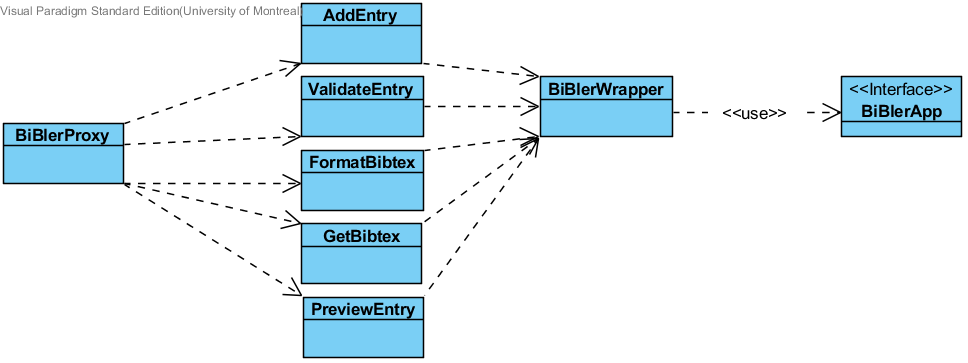
\includegraphics{DomainClassDiagram.png}
\end{figure}

\section{Design}
\subsection{Modélisation}
Le webservice dépend de BiBler et n'utilise que la classe BiBlerApp qui correspond à l'API de cette dernière. Ensuite, le webservice instancie un object BiBlerApp et encapsule chacune des méthodes demandées. Chaque méthode est invoquée par un URL différent. Chacun de ses URLs réfèrent à une classe dont la méthode POST renvoit à la méthode correspondante de BiBler qui est encapsulée par la classe BiBlerWrapper du webservice pour assurer les instanciations locales nécessaires et les appels de méthodes de l'API. Les méthodes de l'API qui n'ont pas été encapsulées sont celles qui effectuent des query dans une application déjà existante qui contient des entrées. Elles pourraient être encapsulées, mais vu le choix de ne conserver aucune donnée, le résultat serait toujours nul. \newline

Il a été décidé que le webservice possèderait deux fichiers. Le premier, application.py, servirait de controlleur afin de rediriger les demandes du client vers les méthodes contenues dans la classe BiBlerWrapper, qui, comme son nom l'indique, servait d'emballeur aux méthodes de la classe BiblerApp du code source de BiBler, ce qui correspond au diagramme de classes suivant, en incluant le Proxy:


\begin{figure}[h!]
\caption{Design logiciel}
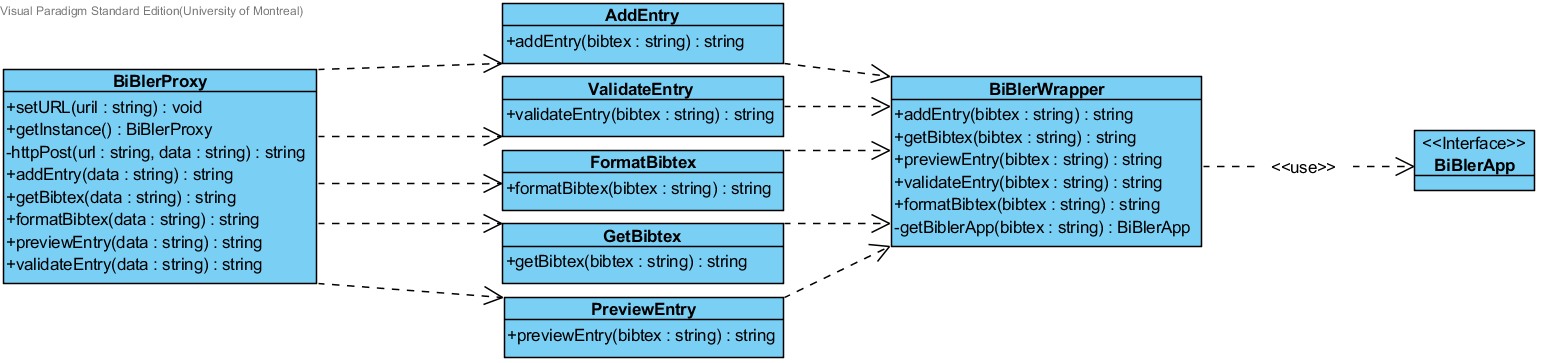
\includegraphics[width=\textwidth,height=\textheight,keepaspectratio]{ClassDiagram.png}
\end{figure}

Au niveau architecturel, les liens entre BiBler, le webservice et ReLiS sont définis tels que présenté dans le diagramme de composantes suivant:


\begin{figure}[h!]
\caption{Diagramme de composantes}
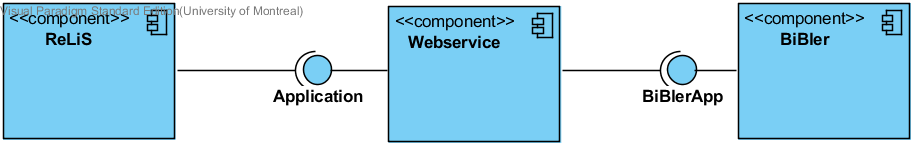
\includegraphics{ComponentDiagram.png}
\end{figure}

Selon les besoins, il fallait étendre les fonctionnalités de BiBler pour accommoder les besoins spécifiques de ReLiS, mais l'interfaçage était déjà présent avec la classe BiBlerApp, il fallait créer de toute pièce le webservice en utilisant l'interface fournie par BiBlerApp et de créer une interface permettant à ReLiS de l'utiliser. Il fallait étendre également ReLiS pour pouvoir utiliser l'interface prochaine du webservice. \newline



\subsection{Justification de l'utilisation de POST vs GET}
Les méthodes POST et GET sont des protocoles http servant au transfert d'information sur le web. On les distingue habituellement par le fait que le protocole GET transmet l'information via l'URI, tandis que le protocole POST cache l'information au moment de la transmission. Dans les faits, plusieurs autres différences font en sorte que l'un ou l'autre des protocoles est mieux adapté à notre cas d'utilisation qui est de soumettre une chaîne de caractère au webservice afin qu'il retourne également une chaîne de caractère au client.\newline

Chacune des méthodes offraient des avantages distincts. La méthode http GET permettait de faire une requête en passant directement les paramètres dans l'url de la requête. Au niveau de la mémoire, c'est également une opération qui peut être mise en cache afin de ne pas renvoyer d'informations inutiles au serveur en cas de requête partielle \cite{w3b}. Sémantiquement, c'est également une opération où l'on demande au serveur de nous fournir de l'information. C'était donc une opération qui semblait initialement correspondre aux besoins du projet. Le méthode http GET a, par contre, une lacune importante quant au transfert de données:

\blockquote {The HTTP protocol does not place any a priori limit on the length of a URI. Servers MUST be able to handle the URI of any resource they serve, and SHOULD be able to handle URIs of unbounded length if they provide GET-based forms that could generate such URIs. A server SHOULD return 414 (Request-URI Too Long) status if a URI is longer than the server can handle (see section 10.4.15).

      Note: Servers ought to be cautious about depending on URI lengths
      above 255 bytes, because some older client or proxy
      implementations might not properly support these lengths. \cite{w3c}
      } 
      
Même si la longueur n'est modulée par les protocoles eux-mêmes, on ne peut être assurer que tout client aura la même expérience en fonction des contraintes des serveurs et proxy impliqués dans les opérations. C'est d'ailleurs ce qui a marqué le glas de la méthode GET au sein du webservice, lorsque des tests préliminaires avec plusieurs entrées BibTeX envoyés en simultanée via le protocole GET n'ont pas retournés de résultat, alors que les mêmes opérations avec le protocole POST retournaient un résultat satisfaisant. Nous entrerons plus en détail dans la section sur les tests de performance à ce sujet. La gestion des configurations des serveurs et proxy du client sont un désagrément suffisant pour ne pas vouloir s'y ingérer et justifie en lui seul l'utilisation de POST. En même temps, POST garantie une plus grande sécurité de l'information, puisque l'information ne transite pas explicitement à par l'URI envoyé. \cite{w3a} Sémantiquement, son utilisation est également justifiable, car même si l'on attend une réponse du serveur, le client lui soumet tout de mêmes une série de données qui doivent être traitées. \newline
\subsection{Stabilité et abstraction}
Si l'on considère seulement le webservice, sans son intégration, il est dépendant de la classe BiBlerApp et aucune classe n'en dépend. Son instabilité est donc de 1 et, comme son abstraction est 0, le webservice est complètement dépendant. Si on le considère dans son intégration, un lien afférent supplémentaire est ajouté du côté de ReLiS, ce qui lui confère un ratio de 1\/2:0, ce qui ne semble pas idéal. Le rôle de médiateur du webservice lui procure une stabilité assez fragile puisqu'il est à la fois dépendant de BiBler et responsable vis-à-vis ReLiS. Par contre, l'idée derrière le webservice est d'interfacer pour le web l'API de BiBler, ce qui fait en sorte qu'une fois l'API dévoilée, la responsabilité incombe plutôt au client pour l'utilisation correcte du service offert. D'un autre côté, si le client est insatisfait, puisque le webservice ne retourne aucun contenu qu'il produit lui-même, le problème ne sera forcément dû au webservice en soi. \newline


\section{Implémentation}
Au sein du fichier application.py,  la variable urls est une collection de paires de strings correspondant respectivant à une URI et à une classe. Les classes présentent jouent le rôle de handler par rapport aux requêtes. La variable app instancie l'application à partir d'une méthode du framework qui prend en paramètre la variable urls et le résultat de la méthode globals$()$ qui représente un dictionnaire du module actuel \cite{PDa}. la variable application instancie l'application à partir de la variable app sur laquelle est appellée wsgifunc(), ce qui permet à l'application d'être déployée sur un serveur Apache 2 sur lequel est installé le module mod\_wsgi qui permet d'instancier des serveurs http à partir de code Python. Pour traiter les données soumises, chacune des classes possèdent une méthode POST qui est appelée lorsque qu'un client soumet une requête http POST à une URL correspondante à une des classes handlers. Chacun des handlers appelle la méthode web.data() qui permet de récupérer les données envoyées via les protocoles web, ce qui permet de récupérer les données du client. Sur ce résultat, on appelle decode() pour transformer l'objet byte-like en string qui être utilisée comme argument pour les méthodes de BiBlerWrapper. Avant d'être soumise, la méthode urllib.parse.unquote\_plus() est utilisée pour parser les espaces et caractères spéciaux qui devraient avoir été encodés du côté client. Toutes les fonctions du package web viennent du framework web.py. \newline

Le fichier bibwrap.py contient la classe BiBlerWrapper dont l'ensemble des méthodes sont statiques. La méthode privée getBiblerApp() est utilisée par les autres méthodes pour générer des instances locales de BiblerApp qui est nécessaire à l'appel de l'ensemble des méthodes. Les méthodes sur les entrées commencent toujours par ajouter une entrée, puis retourne le résultat de la méthode voulue. La classe fait usage du patron de l'emballeur pour encapsuler les méthodes de BiblerApp \newline

L'utilisation attendue du webservice est via une requête http POST vers une méthode du webservice. Dans le cas de ReLiS ou d'un service basé sur PHP, la fonction suivante permet de faire une requête, attendu que \$url contient l'url de la méthode désirée et que \$data contient les données à transmettre sous forme de String: 
\begin{lstlisting}

function httpPost($url, $data)
{

  $ch = curl_init( $url );
  curl_setopt( $ch, CURLOPT_POST, 1);
  curl_setopt( $ch, CURLOPT_POSTFIELDS, urlencode($data));
  curl_setopt( $ch, CURLOPT_FOLLOWLOCATION, 1);
  curl_setopt( $ch, CURLOPT_HEADER, 0);
  curl_setopt( $ch, CURLOPT_RETURNTRANSFER, 1);

  $response = curl_exec( $ch );
    return $response;
}

\end{lstlisting}

Pour encore plus simplifier la chose, le patron de Proxy a été implémenté dans une petite librairie php afin d'encapsuler davantage les requêtes. Une classe Singleton BiBlerPost qui contient un attribut privé URL et un attribut privé instance sert à invoquer les méthodes du webservice et les méthodes publiques de la classe ont le même nom que les classes correspondantes du webservice et ne demandent qu'un argument qui correspond au contenu à envoyer pour traitement. On peut modifier l'URL qui correspond à l'emplacement du webservice avec la méthode setURL qui prend un URI en argument. Des modifications subséquentes au webservice pourrait étendre la classe actuelle afin d'incorporer un plus grand nombre de méthodes ou de modifier le comportement des méthodes actuelles par override afin de correspondre à une modification éventuelle de l'interface fournie par le webservice. Avec le Proxy actuel, le client n'a donc qu'à déterminer l'emplacement web du webservice appelée et à appeler les méthodes désirées sur l'instance unique de la classe. \newline

Pour l'intégration avec ReLiS, un champ abstract a été ajouté au code originel de BiBler. Pour ce faire, abstract a été ajouté à l'énumération des champs possibles. Une classe Abstract héritant de Field a égalément été ajoutée et abstract a été ajouté aux champs possibles de divers éléments, comme Article. Toutes les modifications se retrouvent dans le paquet app de BiBler. \newline

La classe Abstract a été ajoutée au fichier field.py:
\begin{lstlisting}[style=py]
class Abstract(Field):
    """
    The field for the abstract.
    """
    def __init__(self, value = ''):
        super(Abstract, self).__init__(FieldName.Abstract, value)
        
    def format(self):
        self.value = self.value.replace(' ', '')

\end{lstlisting}

Dans fieldname.py, la ligne suivante a été ajoutée dans l'énumération
\textquote{Abstract= 'abstract' \# not part of the BibTeX standard}

À la ligne 26 de app\_interface.py, la variable \textquote{
    Abstract = 'abstract'} a été ajoutée et dans la méthode list(), \textquote{EntryListColumn.Abstract} a été ajouté en fin de liste. Pour terminer, dans entry.py, EntryListColumn.Abstract a été ajouté dans les champs optionnels (attribut self.optionalFields) des différentes classes héritant de Entry.

\section{Tests et documentation}
\subsection{Tests unitaires}
Les cas de tests unitaires étant les mêmes que pour BiBler, les oracles des Tests de BiBler ont été réutilisés pour les tests unitaires du webservice. La batterie de tests est beaucoup plus restreintes, puisqu'une grande partie des méthodes de BiBler n'ont pas été dévoilées dans son webservice. Les tests ont été rédigés grâce au module Pyunit pour Eclipse IDE. Le tout est colligé dans la classe TestAll qui exécute successivement l'ensemble des tests. \newline
\subsection{Tests de performance}
Les performances du webservice ont été testées de façon locale entre le webservice et une application php, tous deux installés sur un serveur Apache 2. L'application php a soumise des requêtes au webservice 10 fois pour chaque pallier décider. Ces palliers sont de 50, 100, 200, 500, 1000 et 2000 requêtes. Le temps requis au webservice pour retourner une réponse à l'application php a ensuite été compilé dans un fichier texte, puis analysé statistiquement. À partir de 3000 requêtes, le temps de réponse commençant à dépasser une minute, le serveur a commencé à renvoyer une erreur service indisponible, qui est la limite de temps permise au niveau de la configuration du serveur Apache utilisé. Le contenu d'une requête typique était @BOOK{, author = {Adams}, publisher = {Bookclub}, title = {H2G2}, year = {1978}, volume = {1} }. \newline

Le temps de réponse moyen par requête a été de 19,91s pour un total de 38500 requêtes envoyées. Les graphiques qui suivent représentent respectivement le temps par nombre de requête et le temps par requête par nombre de requête. Le premier est afficher sur une échelle logarithmique avec un courbe de tendance linéaire. Son coefficient de détermination est de 0.994, ce qui nous montre très clairement que le temps pris était linéaire, même en soumettant 2000 requêtes au webservice. Les points sur le graphique correspondent aux valeurs individuelles des batteries de tests. Le graphique suivant représente le ratio temps par requête selon le nombre de requêtes soumises et les résultats suggèrent que le temps par requête demeure stable même sous un apport important de requêtes. Cette quantité de requêtes en simultanée serait immense pour la portée actuelle du projet, il est donc assez sûr de dire que le webservice devrait avoir des performances stables en environnement de production. Bémol, bien que la machine de test ne soit pas uniquement dédiée au webservice, le fait que les tests soient locaux accélère définitivement le temps de réponse. En contexte de production, la vitesse des réponses variera grandement en fonction de la connexion de l'utilisateur. \newline


\begin{figure}[h!]
\caption{Temps total par nombre de requêtes soumises}
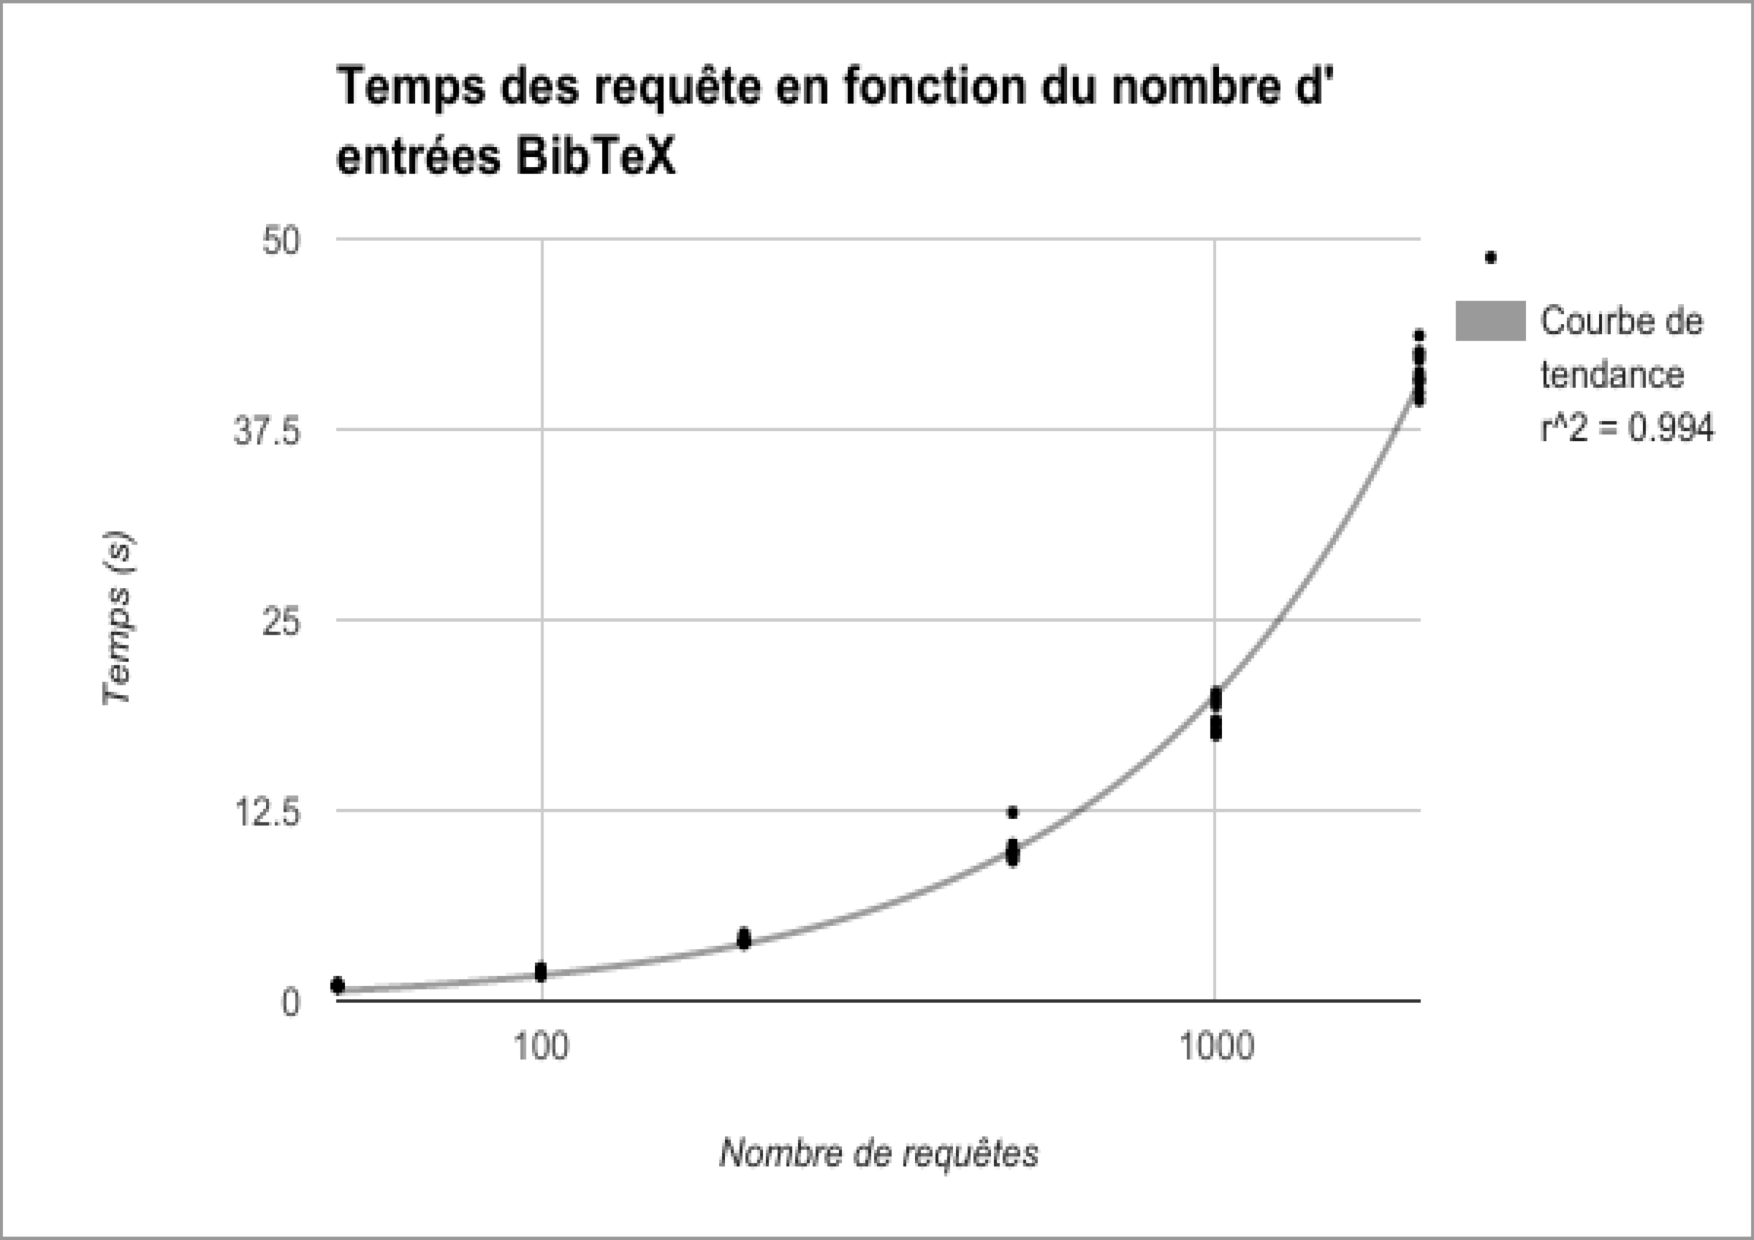
\includegraphics[width=\textwidth,height=\textheight,keepaspectratio]{tempsparrequete.pdf}
\end{figure}

\begin{figure}[h!]
\caption{Temps par requête selon le nombre de requêtes soumises}
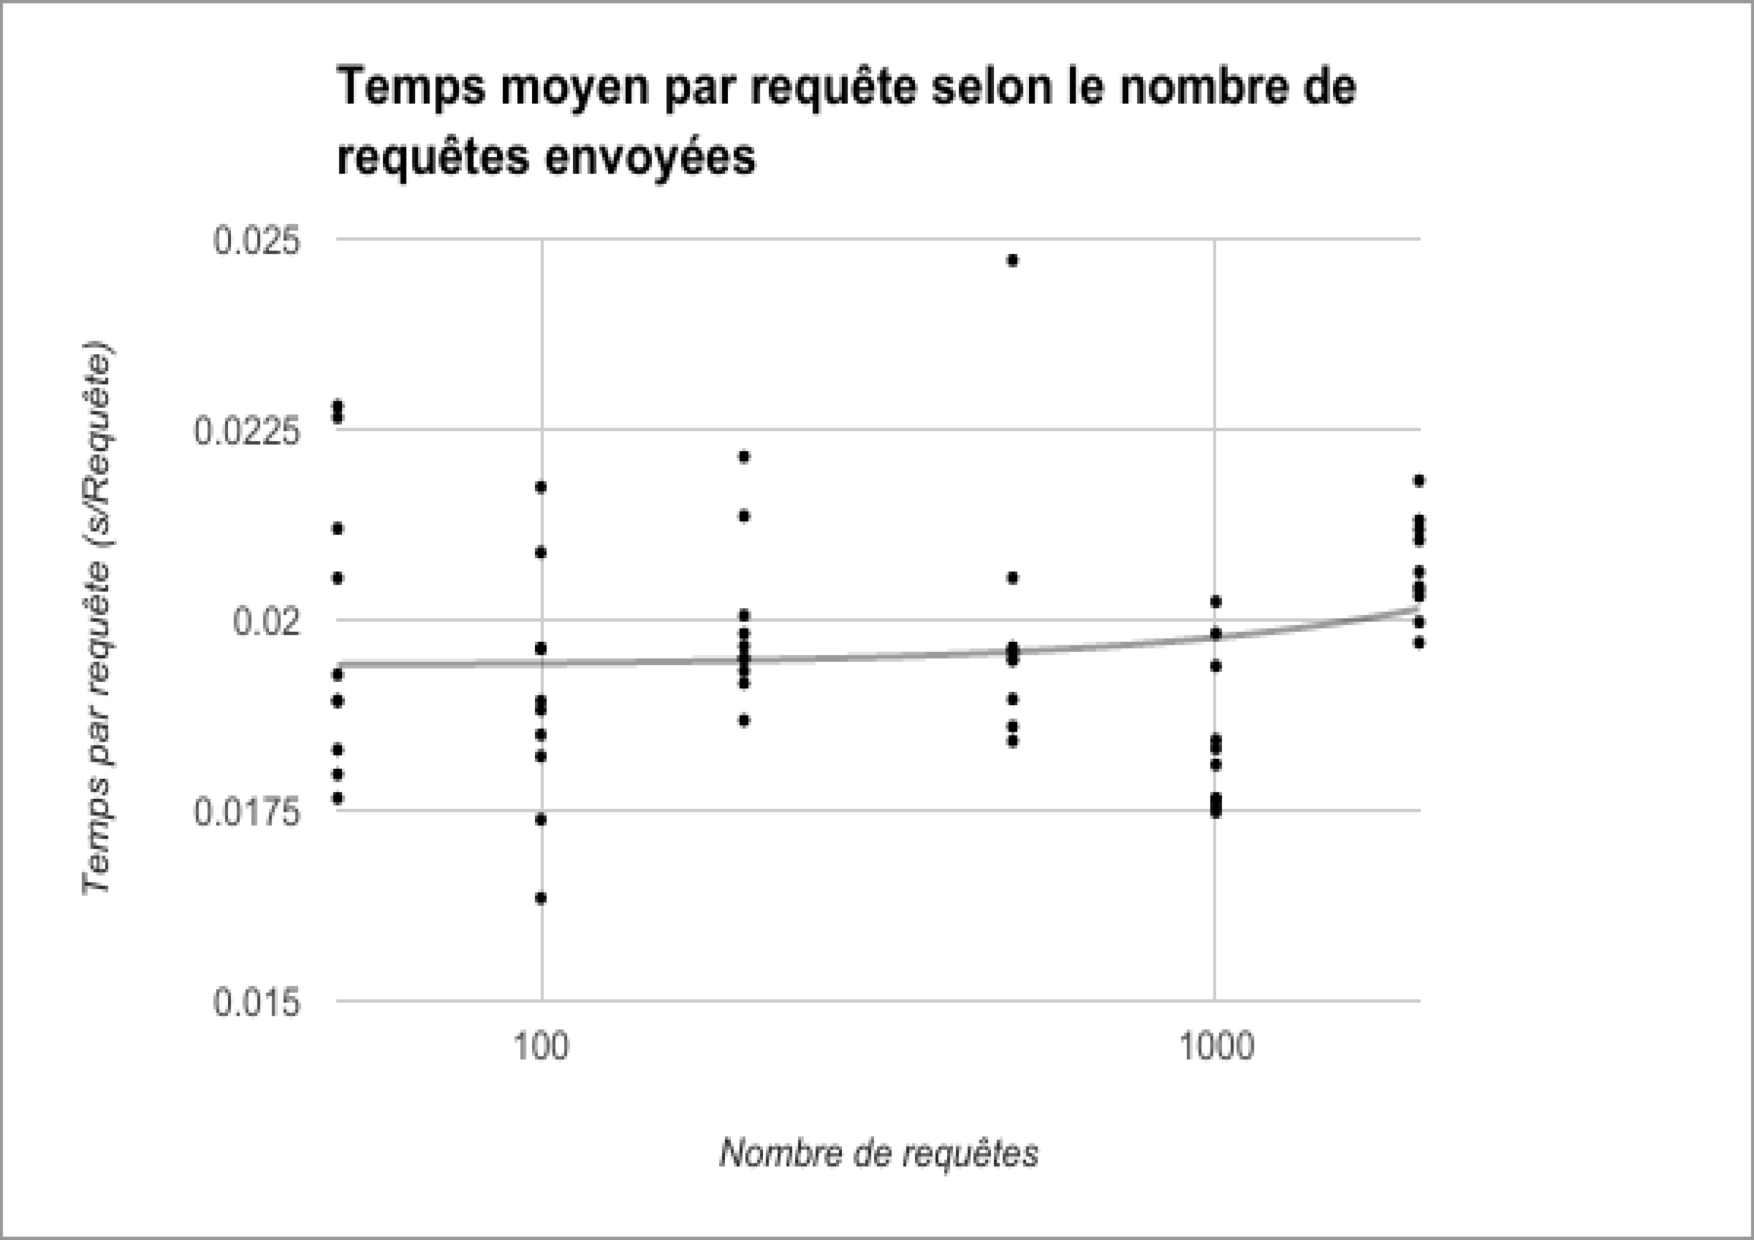
\includegraphics[width=\textwidth,height=\textheight,keepaspectratio]{tempsparequeteparrequete.pdf}
\end{figure}

Il est tout de même intéressant de noter que les écarts-types des valeurs de temps pour un nombre de requêtes données sont de plus en plus restreints à mesure que le nombre de requête grandi, ce qui est certainement causé par un amortissement du poids moyen de chaque requête pour l'ensemble du temps de la requête-mère. La seule donnée probante à ce sujet est que le temps pris par requête à 2000 requête est plus grand que pour 1000 requêtes dans 8 cas sur 10. Considérant l'échelle utilisée, l'écart est tout de même petit, mais les meilleurs performances moyennes par requêtes se retrouvent tout de même dans le cap des 1000 requêtes avec une performance de 18.46s, ce qui est tout de même 1.5s plus rapide que la moyenne globale et 2.2s plus rapide que pour la moyenne sur les tests de 2000 requêtes. On parle tout de même d'une moyenne environ 10\$ plus rapide, ce qui fait des tests à 1000 requêtes 7.26\% plus rapide que la moyenne globale et 10.73\% que la moyenne des 2000 requêtes.

\subsection{Documentation}
La documentation a été rédigée en docstring rst \cite{PDGa}, puis générée avec l'outil Sphinx-python. Une fois la documentation rédigée correctement en rst, Sphinx peut être utilisé. la commande \$ sphinxp-quickstart invoquée dans un terminal créé un répertoire avec une configuration de base pour la génération de la documentation. Le répertoire contient trois sous-répertoires build, Makefile et source. La configuration peut être modifiée au sein du fichier config.py du sous-répertoire source. La commande \$ sphinx-build -b html sourcedir builddir permet de générer les fichiers rst à partir du code source python. Finalement, la commande \$ make html invoquée à partir du répertoire initialement créé par \$ sphinx-quickstart. La dernière commande construit les fichiers html à partir des fichiers compris dans le répertoire source. À partir du fichier index.html, on peut maintenant naviguer la documentation du code source et également choisir de lire des extraits ici du code source. 



\section{Intégration et déploiement}


Les méthodes d'export ont pour attrait de pouvoir envoyer un fichier BibTeX et de le transformer en fichier BibTeX corrigé, en CSV, en HTML ou en SQL. Par contre, cela nécessite l'écriture dans un fichier, ce qui cause problème dans des cas d'écriture en simultanée. Au moment de la rédaction, il avait été choisi de retirer ces fonctionnalités du webservice. Par contre, par l'utilisation du patron d'état, il serait possible d'assurer qu'une seule requête client n'accède au fichier à la fois. Par contre, cela ralentirait nettement la vitesse de retour du webservice puisque les clients demandant l'écriture sur un fichier en cours d'écriture devrait attendre que celui-ci soit disponible afin l'exécution de sa requête.\newline

L'intégration avec ReLiS s'effectue avec un controlleur Bibler.php et une vue frm\_paper\_bibler.php. La vue permet d'instancier un formulaire où les informations sont saisies, puis envoyées au webservice par le controlleur dépendemment de la requête demandée. ReLiS étant basé sur une architecture MVC, le client intéragit avec la vue pour que le controlleur agisse ensuite conséquemment. 

En date du 22 avril, nous étions toujours en attente que le serveur fourni par le DIRO soit accessible pour le déploiement. À ce moment, cela fait plusieurs semaines que le webservice est en attente de déploiement sur les serveurs du DIRO. \newline

\section{Maintenance}
\subsection{Analyse d'impact des modifications sur BiBler}
Avec la demande d'ajout d'un champ au niveau du BibTeX pour l'utilisationde ReLiS, les modifications décrites plus tôt ont été effectuées. L'ensemble de ces modifications sont le fruit d'une analyse du code afin de comprendre les impacts qu'une telle demande a sur la maintenance du code source de BiBler. Le point de départ de l'analyse se trouve au niveau de l'enum FieldName, tel que suggéré par Eugène Syriani lors des discussions initiales sur cette demande de changement. \newline

Le type de changement demandé est incrémental et perfectif. La requête de changement était d'ajouter le champ abstract dans le fichier BibTeX. Les concepts principaux associés à cette requête sont ajouter, champ et abstract. La recherche associée au sein du code source a été au niveau de la classe Field et de son contexte d'utilisation. C'est pourquoi, il a également fallu modifié les classes utilisant field pour incorporer le champ abstract et ajouter abstract à un enum. Au final, l'impact était assez localisé, ce qui a permis de faire les changements rapidement, même si l'impact était tout de même plus grand que ce qui avait été initialement pensé. \newline
\begin{figure}[h]
\caption{Impact du changement}
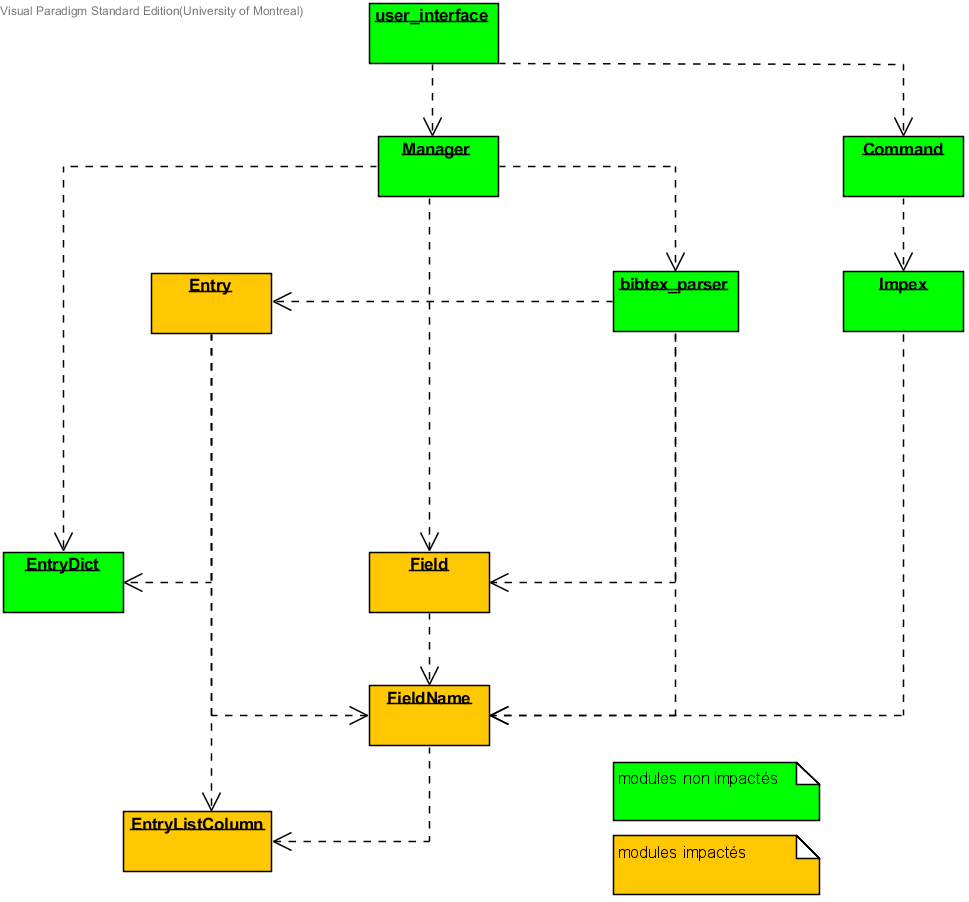
\includegraphics[width=\textwidth,height=.8\textheight,keepaspectratio]{impact.png}
\end{figure}

Le DIP étant très bien respecté en s'éloignant des modules fortement couplés field, field\_name et entry, on se rend compte très rapidement que les autres modules n'ont pas besoin de modifications. Les ajouts ont majoritairement consisté d'une ligne dans chacune des classes impactées pour ajouter la possibilité d'un champ Abstract. Par contre, cela impliquait également l'ajout d'une classe Abstract. Bien entendu, ce nom porte à confusion, mais comme toutes les classes hériant de Field étaient également nommées directement par leur étiquette, il a été décidé de conserver ce nom pour éviter de plus amples confusions. Le champ a été ajouté à chaque classe héritant de Entry parmi les champs optionnels. \newline

\begin{figure}[h]
\caption{Ajout de classe}
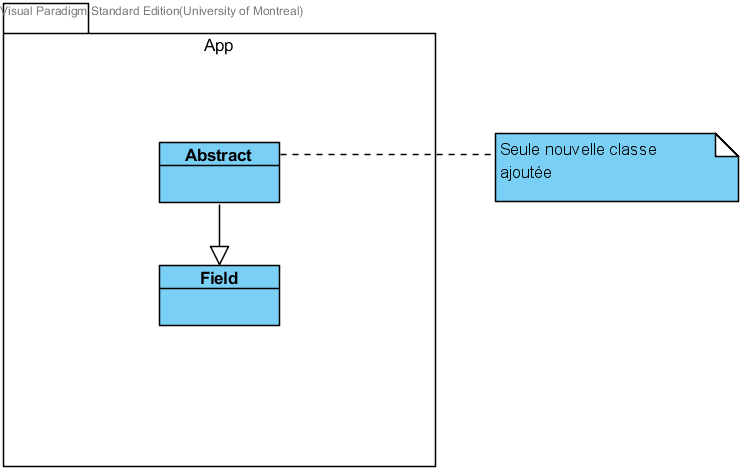
\includegraphics[width=\textwidth,height=.5\textheight,keepaspectratio]{maintenance.png}
\end{figure}

\subsection{Maintenance du webservice}
L'extension du webservice pourra se faire de plusieurs façons. Par exemple, si l'on ne désire pas ajouter au code source de BiBlerWrapper, on pourra toujours hérité de cette classe et ajouter les nouvelles fonctions nécessaires. Du côté du Handler, on n'aura qu'à utiliser les mêmes méthodes qu'auparavant, mais sur la nouvelle classe. Similairement, le Proxy est extensible par polymorphisme. Dans tous les cas, l'ajout de fonctionnalités peut passer par modification du code actuel ou par extension. Les extensions possibles sont principalement au niveau du dévoilement par le wrapper d'un plus grand nombre de fonctions de l'API, ce qui découlerait d'une modificiation de celle-ci ou d'un changement conceptuel au fonctionnement du webservice.


\section{Conclusion}
L'ensemble du projet a été fort intéressant. Bien que le webservice ait pu être réalisé, son déploiement a été laissé de côté en attendant que le serveur devant l'héberger soit en fonction. D'autres contretemps, comme l'erreur fatale de la mise à jour de Manjaro, ont ralentis les avancées prévues. Malgré tout cela, Les fonctionnalités de BiBler sont prêtes à être utiliser à travers le web et une librairie PHP est disponible pour aider les développeurs, même si l'intégration avec ReLiS n'a pas été entièrement complétée. Au final, le travail fait n'est pas perdu et les ressources produites resteront disponibles.\newline

Pour le futur, il serait intéressant d'intégrer les fonctionnalités omises de BiBler par les contraintes d'écriture. Également, le webservice pourrait éventuellement intégrer des sessions afin de permettre à un utilisateur spécifique de conserver en mémoire les entrées ajoutées pour le cours d'une session, sans toutefois intégrer de base de données au webservice. Le format actuel par requêtes http POST permet une grande flexibilité pour l'avenir du webservice de demeure ouvert à l'extension, tel que suggéré dans le workflow de maintenance.

\subsection{Remerciements}

Ce projet m'a permis de toucher à PHP, Python, Apache, Sphinx, Pydev, BiBler, ReLiS et LaTeX. Les apprentissages ont été importants et infiniment intéressants. Python est un langage polyvalent et qui fait preuve d'une grande élégance syntaxique et possède des propriétés intéressantes sur la plan fonctionnel, impératif et orienté-objet. Je travaillerai prochainement au Laboratoire de Santé Publique du Québec où se trouvent une grande concentration d'experts en santé publique et il est certain que ceux-ci pourraient être intéressés par des outils tels que BiBler et ReLiS qui ont un grand potentiel d'automatisation dans un contexte de recherche scientifique.

Les diagrammes ont été créés à l'aide de Visual Paradigm et les graphes statistiques exportés depuis Google Spreadsheets.\newline
Un merci infini à ceux qui m'ont aidé et accompagnés dans cette tâche: \newline
Eugène Syriani, Ph.D., pour la supervision et les conseils précieux\newline
Brice-Michel Bigendak, pour ReLiS et le débogage en PHP,
L'équipe technique du DIRO, pour le support technique et le serveur
\bibliography{references}{}
\listoffigures
\bibliographystyle{plain}
\end{document}
















